\providecommand{\main}{../../../..}
\documentclass[\main/dresen_thesis.tex]{subfiles}
\begin{document}
  \label{sec:doubleLayers:pnr}
  Write something
  % \begin{table}[!htbp]
  %   \centering
  %   \caption{\label{tab:looselyPackedNP:nanoparticle:gisaxs}Parameters for the hard-sphere structure factor in Percus-Yervick approximation shown in \reffig{fig:looselyPackedNP:layer:gisaxs} for both SC-IOS-11 and SC-IOS-7. $R_\mathrm{HS}$ is the hard-sphere radius and $\eta$ the packing fraction of the structure factor.}
  %   \begin{tabular}{ c | l | l }
  %     \rule{0pt}{2ex} \textbf{GISAXS}  & \textbf{SC-IOS-11} & \textbf{SC-IOS-7} \\
  %     \hline
  %     \rule{0pt}{2ex} $R_\mathrm{HS} \, / \unit{nm}$          & $5.655(2)$           & $3.872(4)$\\
  %     \rule{0pt}{2ex} $\eta          \, / \unit{\%}$          & $43.88(3)$           & $34.20(9)$\\
  %     \hline
  %   \end{tabular}
  % \end{table}


  \begin{figure}[tb]
    \centering
    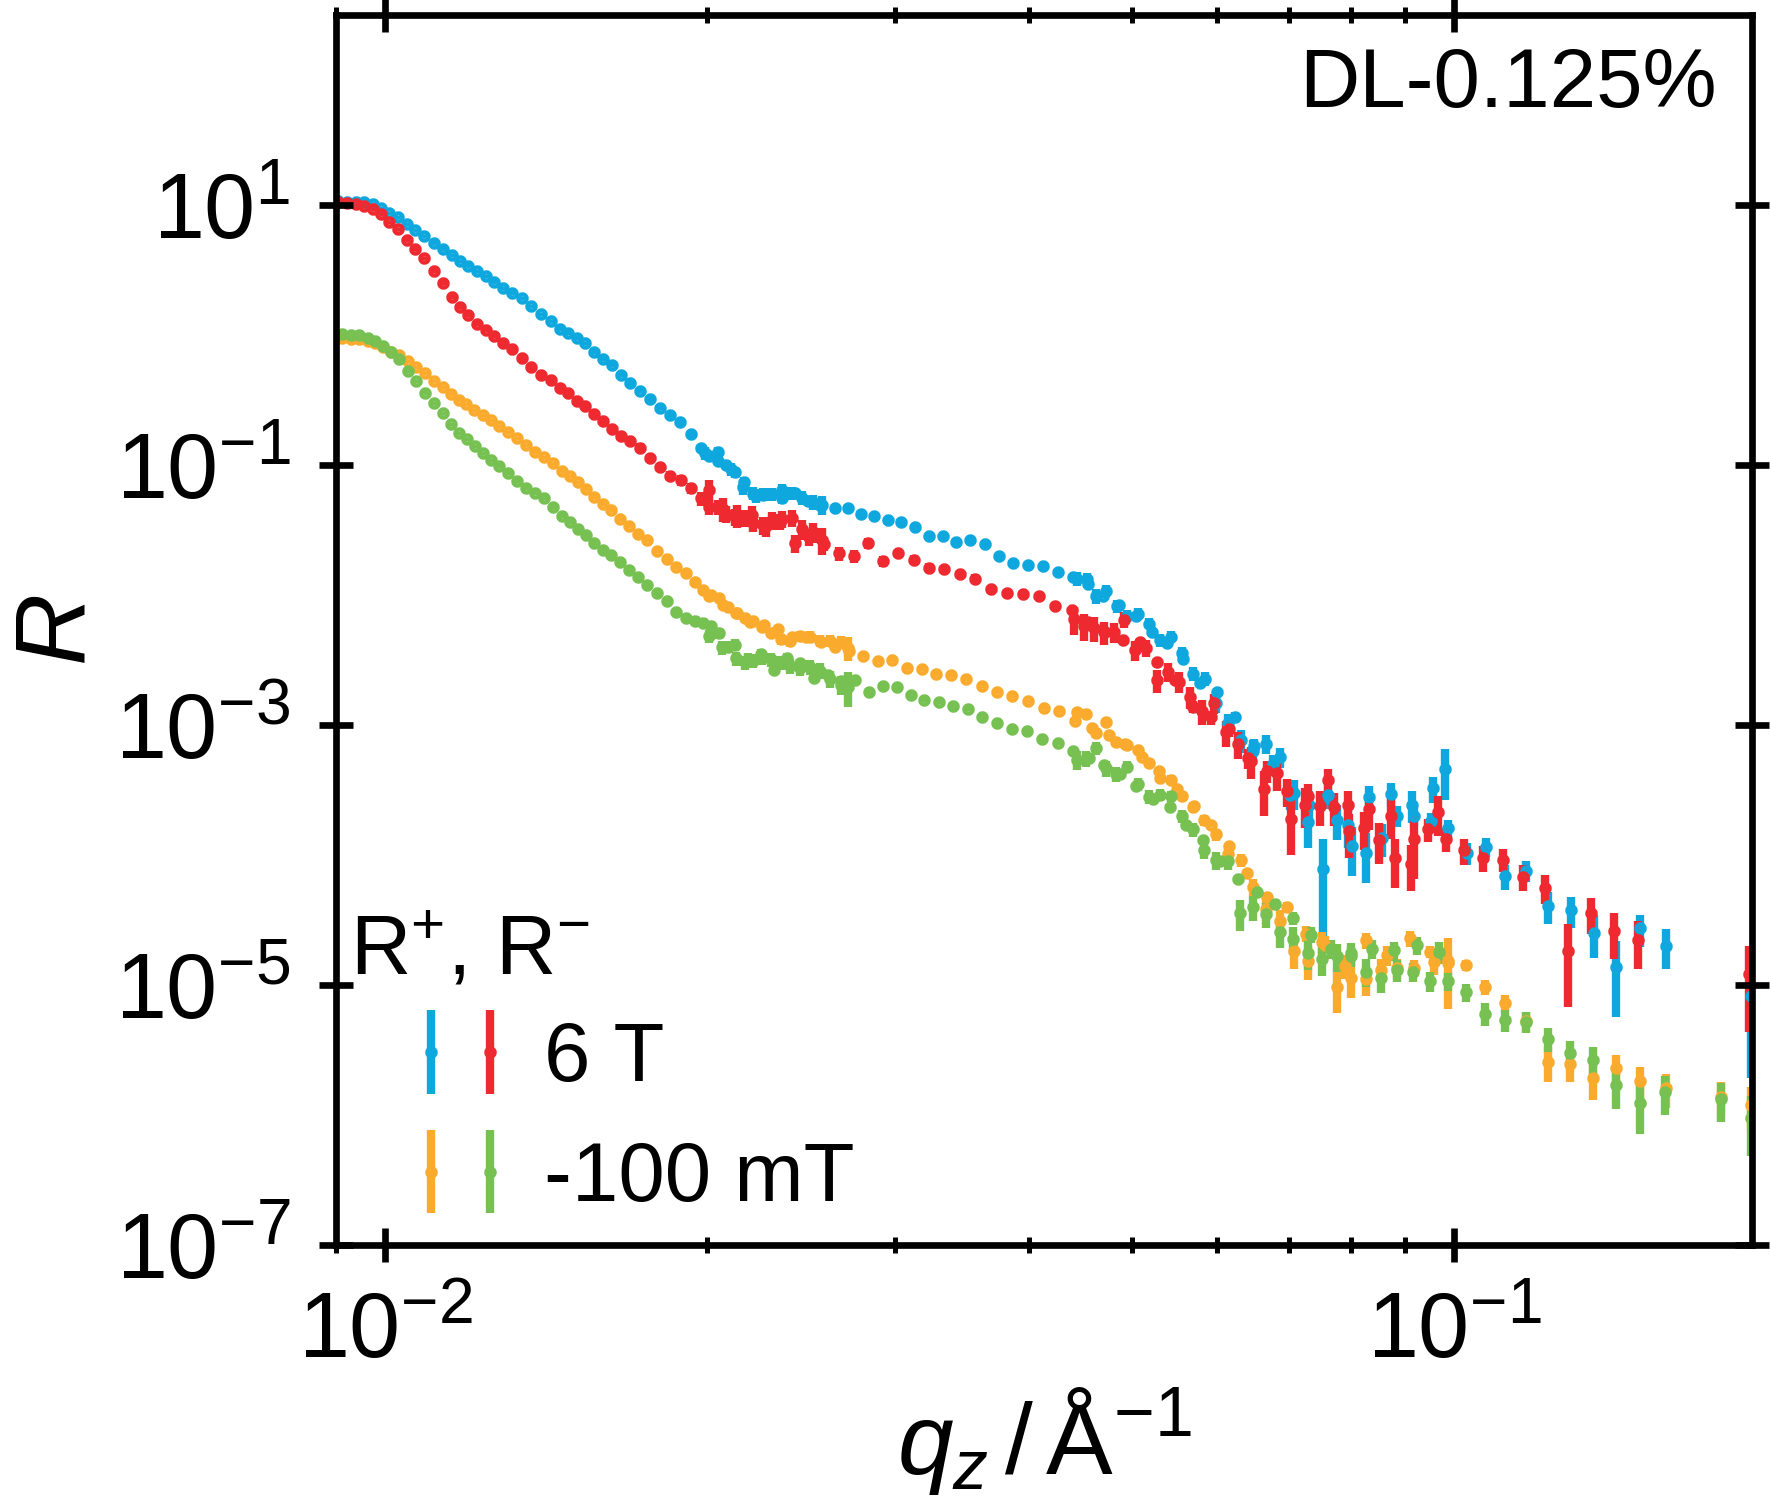
\includegraphics{doubleLayers_VerticalStructure_DL-0-125_PNR_ZFC5K}
    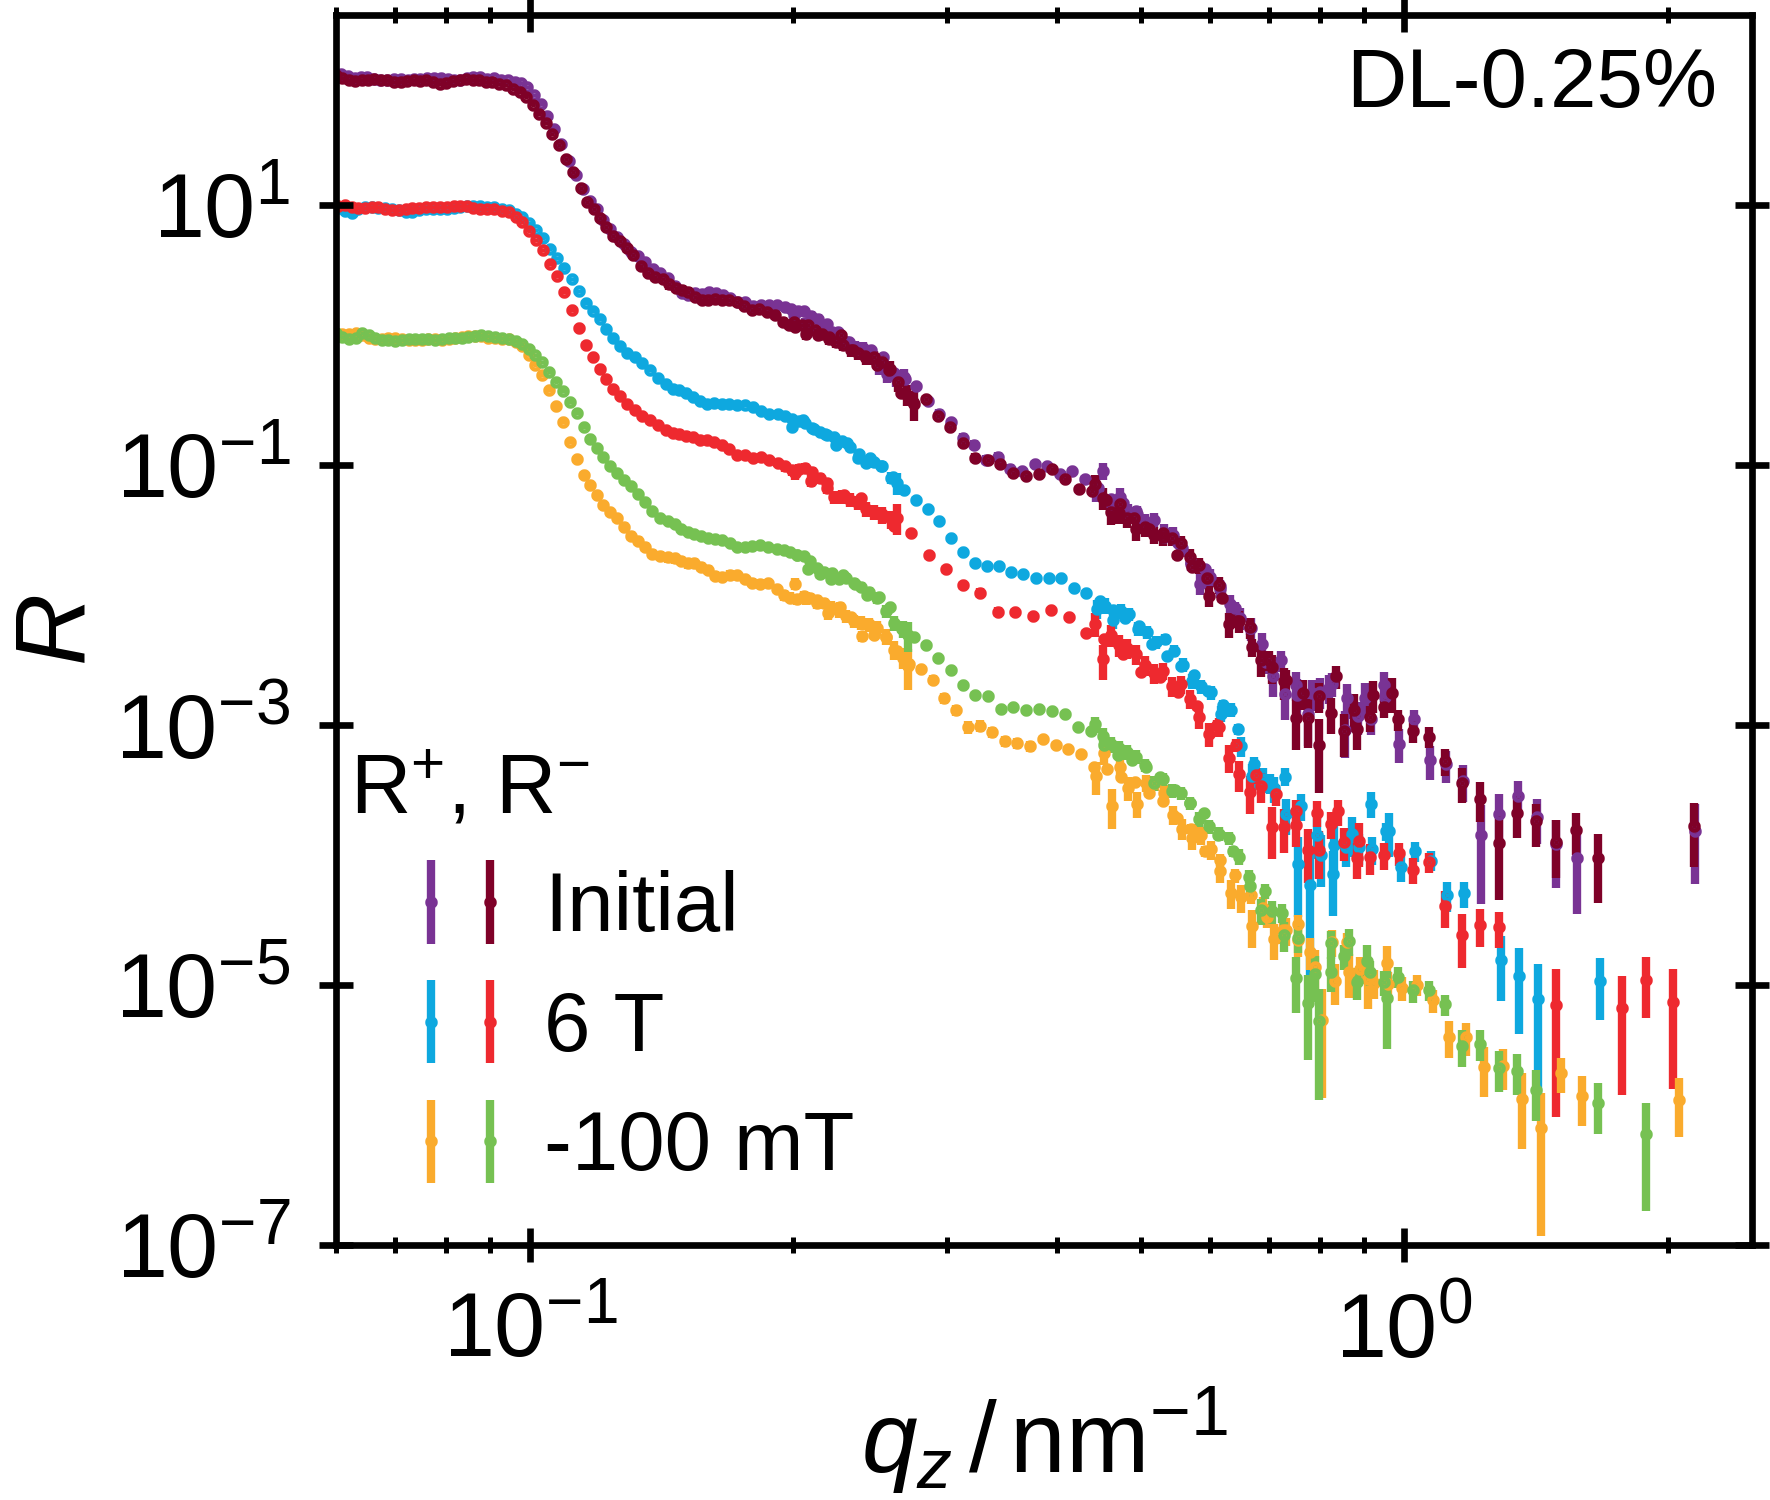
\includegraphics{doubleLayers_VerticalStructure_DL-0-25_PNR_ZFC5K}
    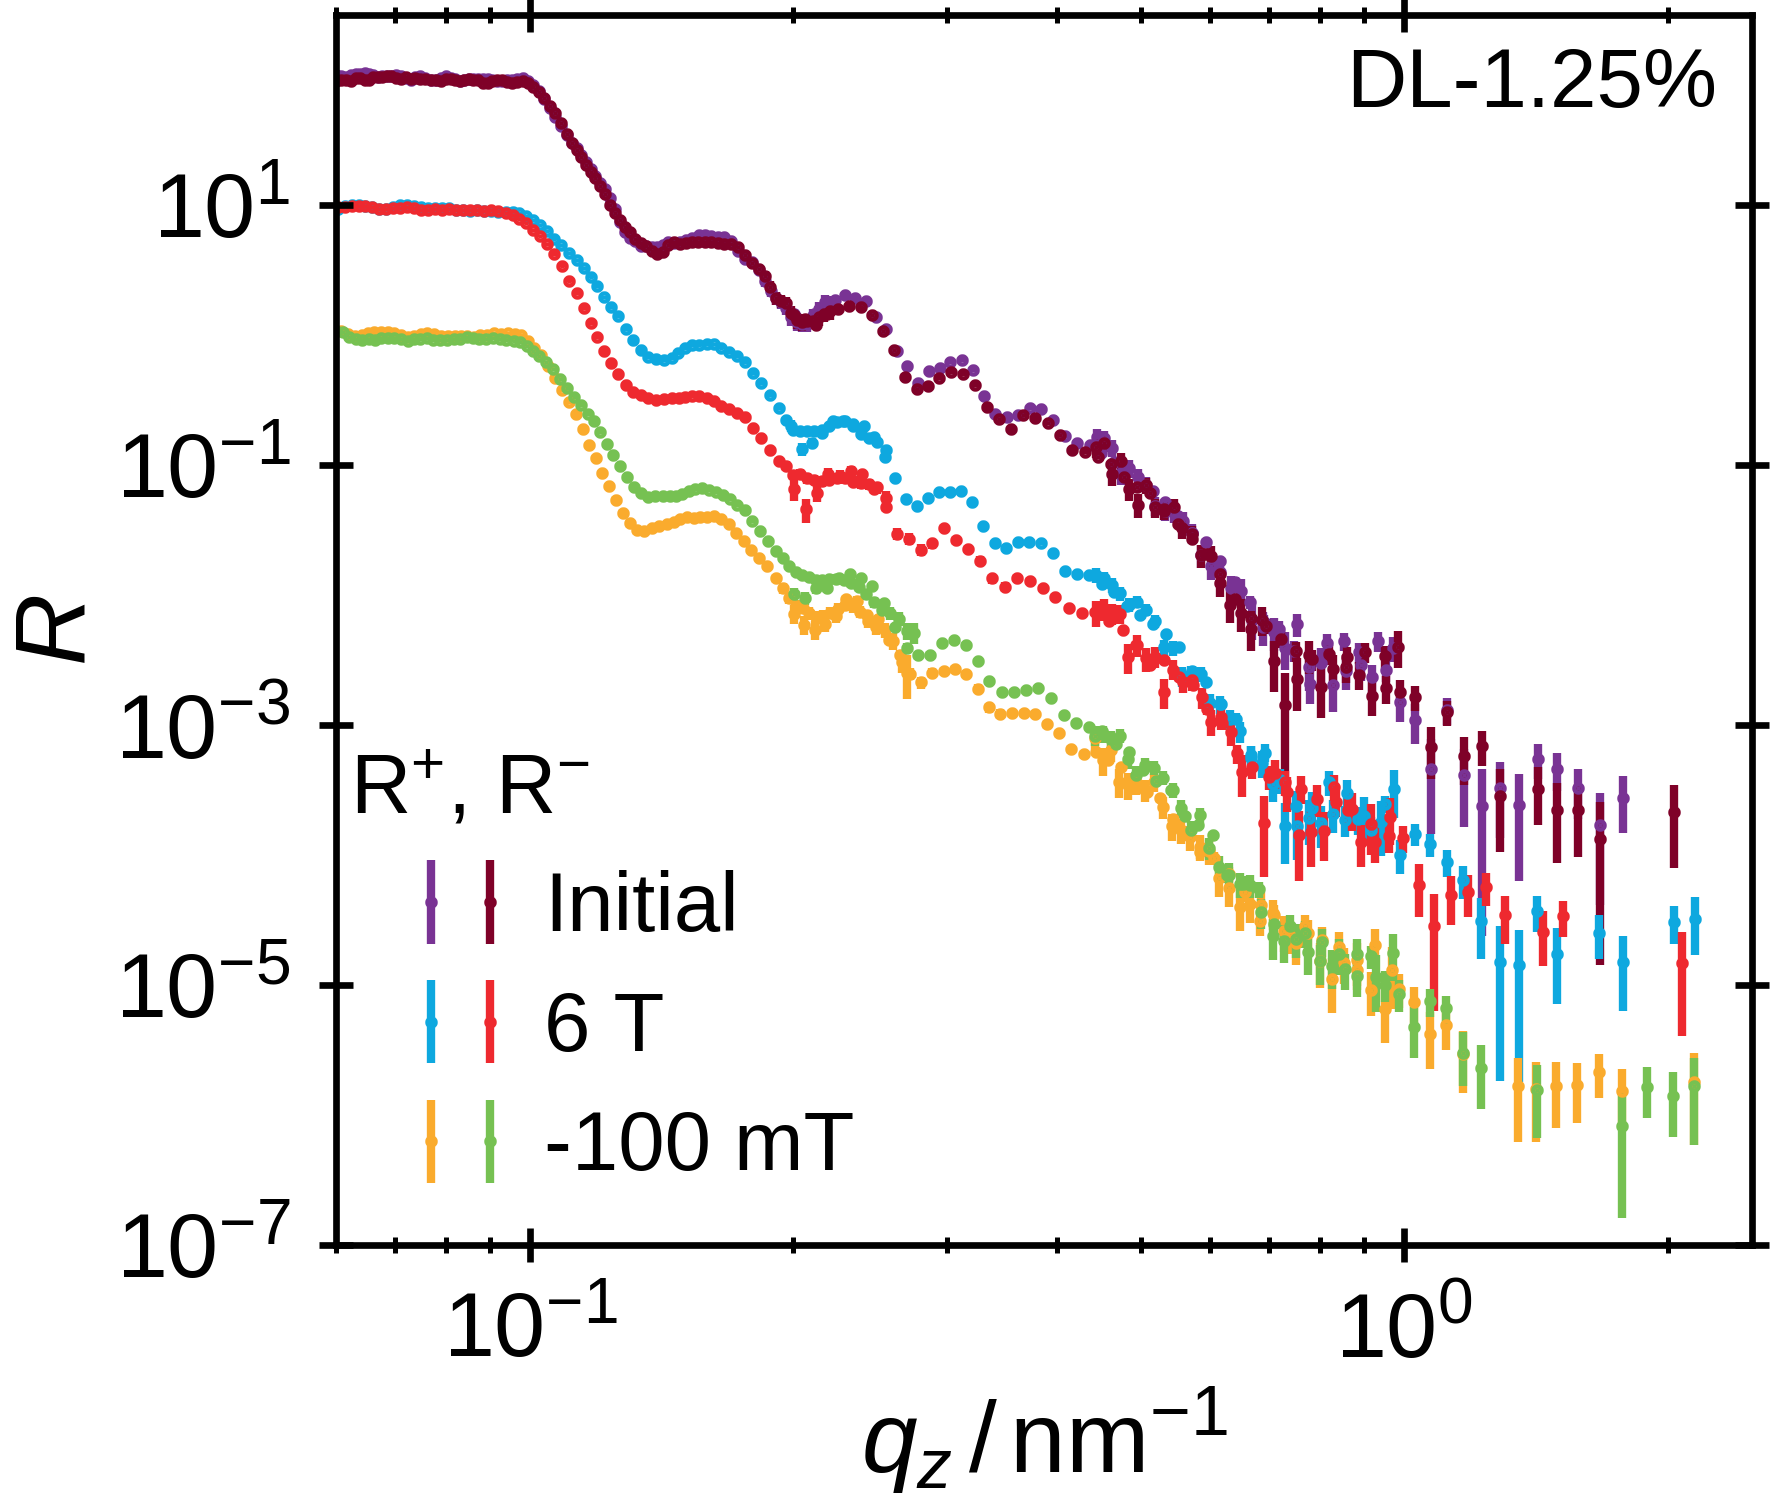
\includegraphics{doubleLayers_VerticalStructure_DL-1-25_PNR_ZFC5K}
    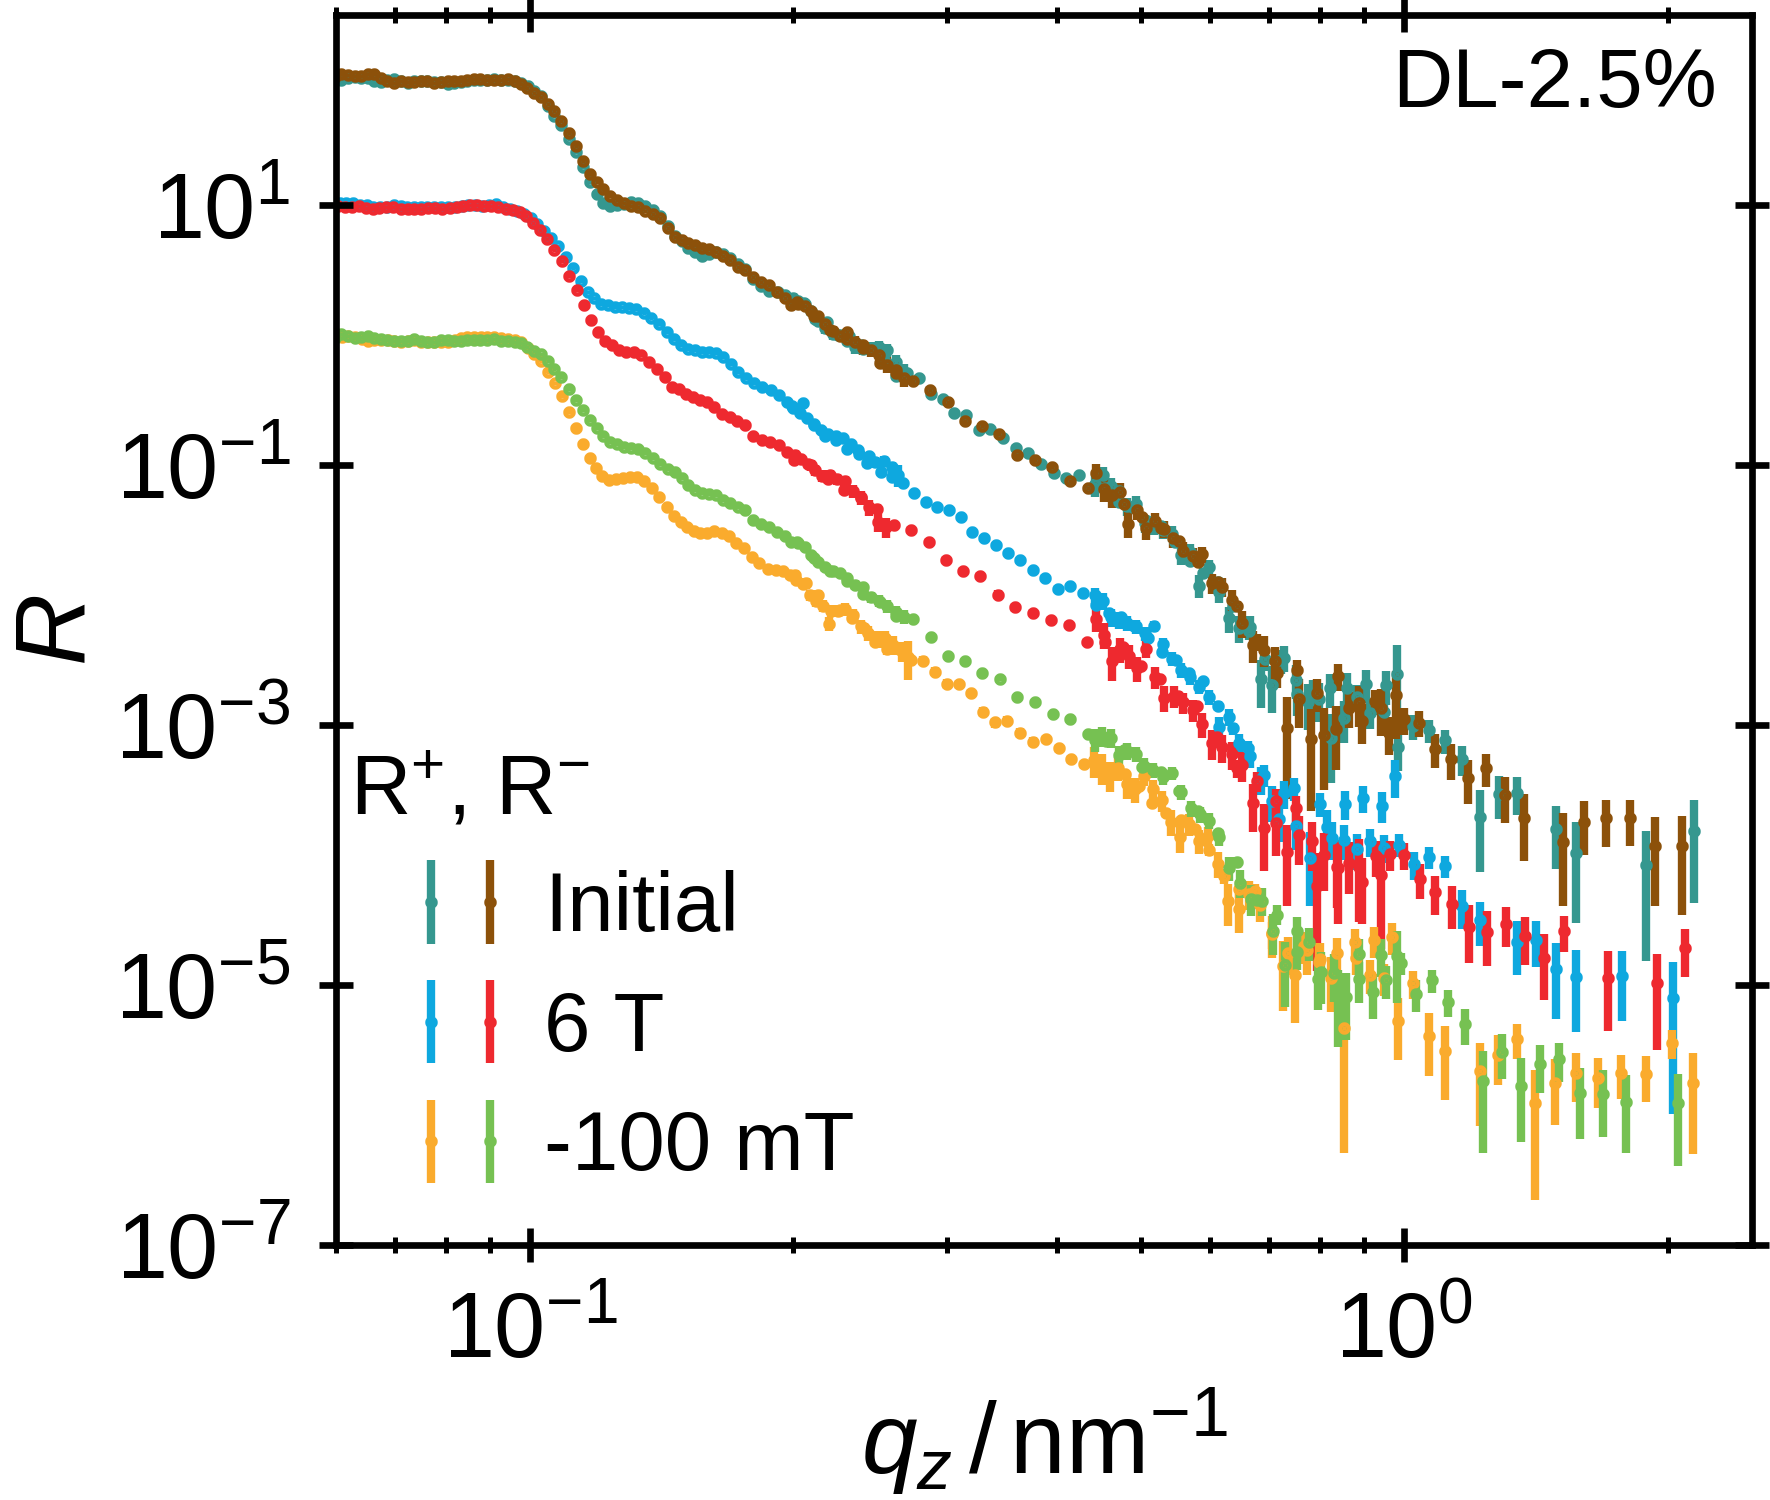
\includegraphics{doubleLayers_VerticalStructure_DL-2-5_PNR_ZFC5K}
    \caption{\label{fig:doubleLayers:pnrData}Polarized neutron reflectometry of DL-0.125\%, DL-0.25\%, DL-1.25\% and DL-2.5\% measured at $5 \unit{K}$ after zero-field cooling. For all samples but DL-0.125\%, the reflectivity at guide field after cooling is shown and furthermore for all samples, measurements at a field of $6 \unit{T}$ and subsequently $-100 \unit{mT}$ are displayed.}
  \end{figure}

\end{document}